\section{Results}

\subsection{Fishery Commons as a signal-design precursor}

The Fishery Commons study is retained as the controlled precursor rather than the center of gravity of the follow-up. Its role is to show that the benchmark can rank central interventions under repeated strategic turnover. In the matched baseline, monitoring with sanctions reduces held-out collapse relative to no governance under both mutation and live JSON-based LLM injection. In the broader non-LLM top-down sweep, adaptive quotas emerge as the strongest overall signal in the medium tier. Across balanced and adversarial-heavy populations, pressures \(0.3\) and \(0.5\), and three non-LLM injector families, adaptive quotas win every injector block while temporary closures remain a credible ecological fallback. A medium-tier PPO validation recovers the same qualitative ordering. The precursor conclusion is therefore narrow but informative: central governance signals can be ranked under capability escalation, and adaptive quotas are the strongest top-down intervention in the simpler substrate.

\begin{table}[t]
  \centering
  \caption{Fishery Commons precursor summary. Collapse reductions are measured relative to no governance in the medium-tier non-LLM sweep. The final column reports the welfare advantage of adaptive quotas over temporary closures.}
  \label{tab:fishery_precursor}
  \small
  \begin{tabular}{@{}lcccc@{}}
    \toprule
    Injector & Sanctions & Adaptive quota & Closure & Adaptive quota minus closure welfare \\
    \midrule
    Mutation & 0.3737 & 0.9167 & 0.9167 & 2408.81 \\
    Adversarial heuristic & 0.0208 & 0.9167 & 0.9167 & 2211.61 \\
    Search over mutations & 0.2617 & 0.9167 & 0.9167 & 2723.02 \\
    \bottomrule
  \end{tabular}
\end{table}

\subsection{Architecture restoration}

The architecture-restoration pilot broadens Harvest Commons from the earlier narrow pairwise comparison to the full architecture spectrum. In the pilot, \texttt{hybrid} ranks first in 6 of 8 decision cells and \texttt{top\_down\_only} ranks first in the remaining 2. Neither \texttt{bottom\_up\_only} nor \texttt{none} ranks first. This already answers the first pilot question: \texttt{bottom\_up\_only} is not redundant with \texttt{none}. Relative to \texttt{none}, bottom-up-only governance improves patch health in 6 of 8 cells and is non-worse on neighborhood overharvest in 6 of 8, although its mean welfare delta is negative. Local coordination therefore contributes something real, but not enough to recover the ecological control achieved by architectures with central intervention.

The broader pilot also clarifies what hybrid governance adds. Relative to \texttt{top\_down\_only}, the pilot yields positive patch-health deltas in 6 of 8 cells and non-worse neighborhood-overharvest deltas in 6 of 8, with a mean welfare delta of only \(-0.0572\). Relative to \texttt{bottom\_up\_only}, both governed architectures buy large patch-health gains but at much larger welfare cost. The pilot interpretation is therefore that local-only governance is empirically distinct, top-down control is ecologically necessary, and the central question is whether hybrid governance adds enough to justify itself over central-only control.

\subsection{High-power architecture confirmation}

The confirmatory Stage C matrix answers that question cleanly. Under the lexicographic failure-then-patch-health-then-welfare rule, \texttt{hybrid} ranks first in all 8 decision cells. \texttt{top\_down\_only} ranks second in every cell, and \texttt{bottom\_up\_only} ranks third in every cell.

The most important comparison is \texttt{hybrid - top\_down\_only}. In the high-power matrix, hybrid improves patch health in all 8 cells, is non-worse on neighborhood overharvest in 6 of 8 cells, and has a mean welfare delta of \(-0.1363\). That welfare cost remains inside the planned \(-0.15\) threshold, so the confirmatory gate is satisfied. The mean patch-health delta is \(+0.0477\), and the mean neighborhood-overharvest delta is \(-0.0813\). The architecture result is therefore not that hybrid dominates every metric in every cell. It is that, under stronger search-based capability escalation, hybrid is the best overall architecture by the study's ranking rule and achieves that rank primarily through ecological and behavioral margins rather than through a collapse-vs-no-collapse effect.

The full architecture spectrum clarifies the mechanism underlying that result. Relative to \texttt{bottom\_up\_only}, both \texttt{hybrid} and \texttt{top\_down\_only} improve patch health in all 8 cells, but both do so with large welfare costs. In the confirmatory matrix, \texttt{hybrid - bottom\_up\_only} has mean patch-health delta \(+3.1234\) and mean welfare delta \(-1.2231\), while \texttt{top\_down\_only - bottom\_up\_only} has mean patch-health delta \(+3.0757\) and mean welfare delta \(-1.0868\). Local-only governance therefore retains more welfare on average, but it does so by tolerating weaker ecological control and nonzero failure risk. Central intervention is necessary, and hybrid governance then improves on central-only control enough to rank first in every confirmatory cell.

\begin{figure}[t]
  \centering
  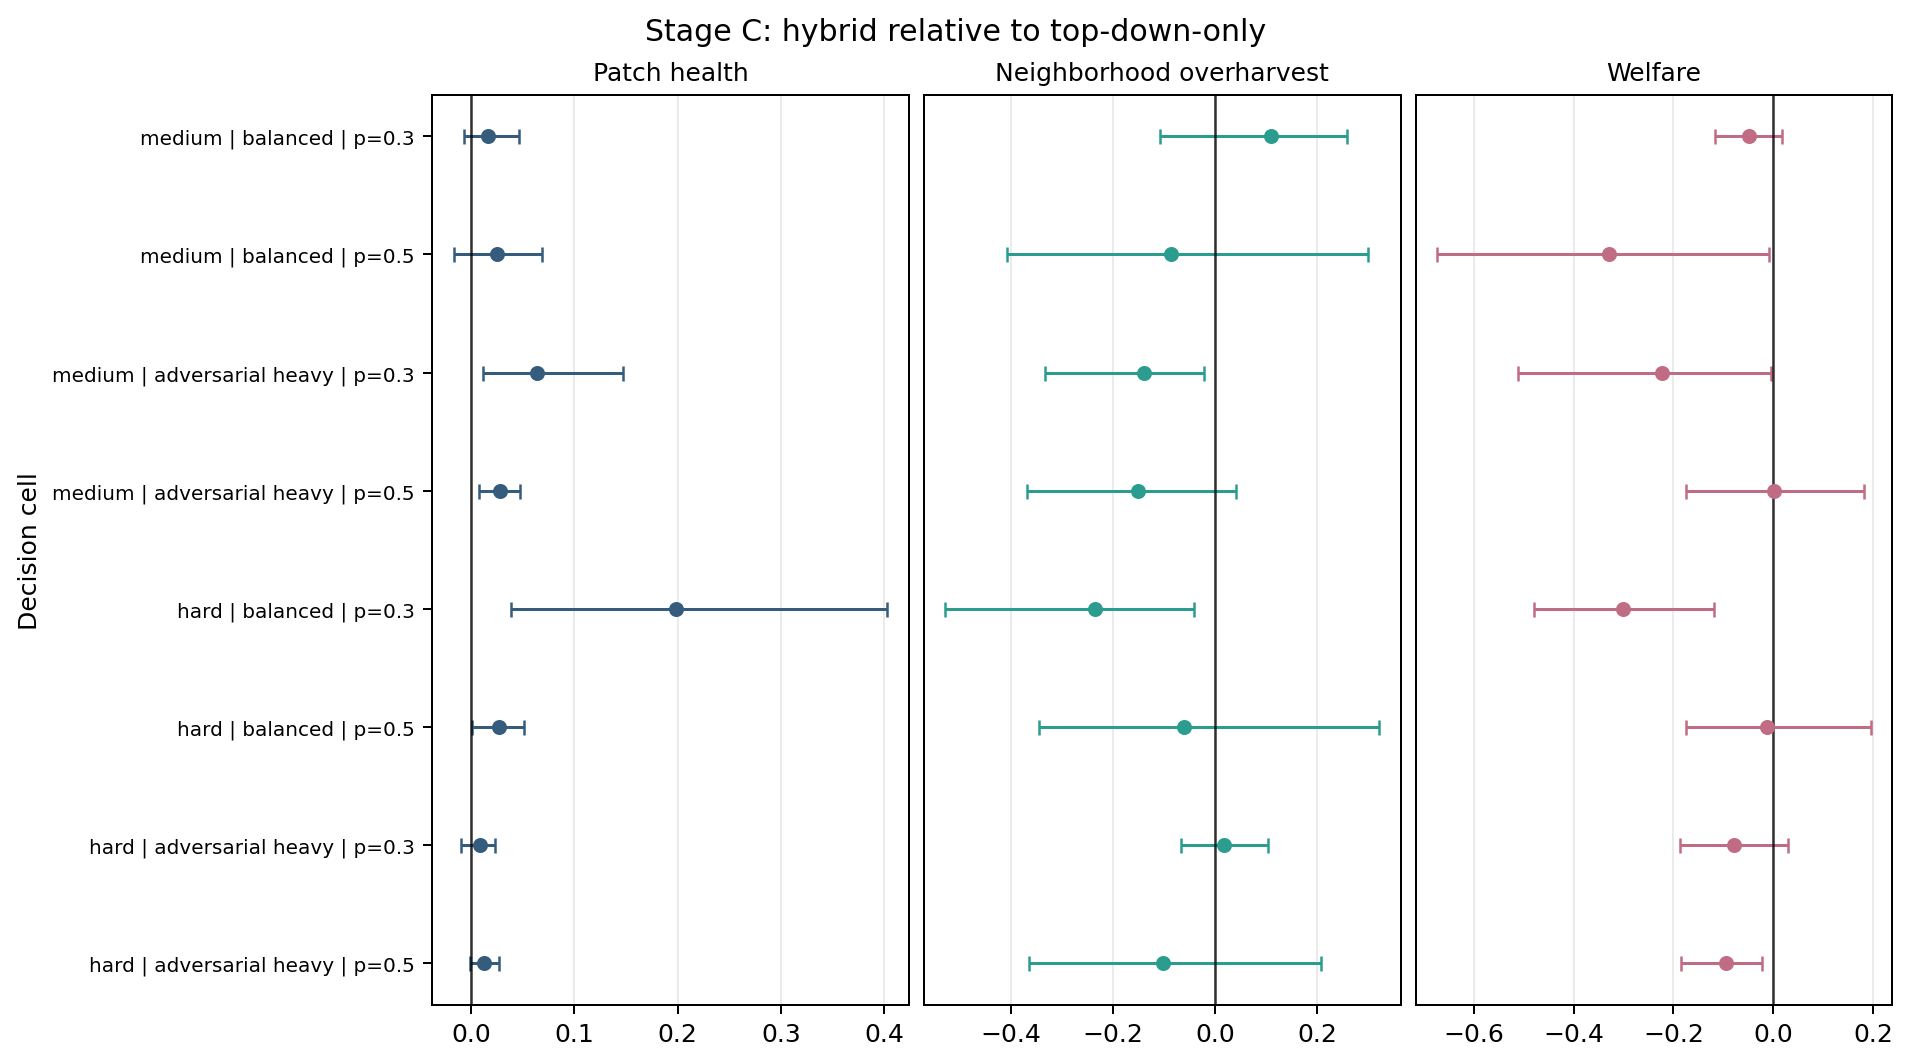
\includegraphics[width=\linewidth]{figures/harvest_architecture_stageC_architecture.png}
  \caption{Cell-level Stage C effect sizes for \texttt{hybrid - top\_down\_only} under \texttt{search\_mutation}. The high-power matrix covers the medium and hard tiers, balanced and adversarial-heavy populations, and pressures \(0.3\) and \(0.5\). Hybrid governance ranks first in every decision cell under the failure-then-patch-health-then-welfare rule, with the margin carried by patch health, neighborhood overharvest, and a moderate welfare cost.}
  \label{fig:harvest_architecture}
\end{figure}

\begin{table}[t]
  \centering
  \caption{Harvest Commons architecture summary. Stage B is the restoration pilot over four governance conditions; Stage C is the high-power confirmatory comparison over \texttt{bottom\_up\_only}, \texttt{top\_down\_only}, and \texttt{hybrid}. Positive patch-health deltas favor the left condition; nonpositive overharvest deltas are improvements for the left condition.}
  \label{tab:harvest_architecture}
  \small
  \begin{tabular}{@{}llrrrr@{}}
    \toprule
    Stage & Contrast & Cells & Patch \(> 0\) & Overharvest \(\le 0\) & Mean welfare \\
    \midrule
    B & bottom\_up\_only $-$ none & 8 & 6 & 6 & -0.3425 \\
    B & hybrid $-$ top\_down\_only & 8 & 6 & 6 & -0.0572 \\
    C & hybrid $-$ top\_down\_only & 8 & 8 & 6 & -0.1363 \\
    C & hybrid $-$ bottom\_up\_only & 8 & 8 & 0 & -1.2231 \\
    C & top\_down\_only $-$ bottom\_up\_only & 8 & 8 & 0 & -1.0868 \\
    \bottomrule
  \end{tabular}
\end{table}

\subsection{Capability ladder}

The capability ladder provides an additional robustness test on top of the Stage B and Stage C architecture results. Across the 32 ladder cells, \texttt{hybrid} ranks first in 25 and \texttt{top\_down\_only} ranks first in the remaining 7. By injector rung, hybrid wins all 8 random cells, 6 of 8 mutation cells, 4 of 8 adversarial-heuristic cells, and 7 of 8 search-over-mutations cells. The ladder therefore does not support a claim that one architecture dominates unconditionally at every rung. It does show that the architecture ordering remains informative under rising pressure, and that the vulnerable comparison is specifically \texttt{hybrid} versus \texttt{top\_down\_only}, not governed architectures versus local-only governance.

That asymmetry is explicit in the first-break table. For \texttt{hybrid - bottom\_up\_only}, the ecological break never occurs in any of the 8 decision cells: the first ecological-break rung is \texttt{none} in all 8. The same is true for \texttt{top\_down\_only - bottom\_up\_only}. In other words, both governed architectures retain their patch-health advantage over local-only governance throughout the full non-LLM attacker ladder. The break points appear elsewhere. In the \texttt{hybrid - top\_down\_only} comparison, the ecological margin survives through the full ladder in 3 of 8 cells, first breaks at mutation in 2, at the adversarial-heuristic rung in 2, and at search over mutations in 1. The control margin follows a similar pattern: no control break in 3 cells, mutation as the first break in 1, adversarial heuristic in 3, and search over mutations in 1.

The ladder also clarifies the role of welfare. The costly-robustness flag trips earlier than the ecological break in the \texttt{hybrid - top\_down\_only} contrast: the first welfare-threshold crossing appears already at the random rung in 6 of 8 cells, at search over mutations in 1, and never in 1. By contrast, the local-only comparisons are ecologically decisive but welfare-expensive from the start. For \texttt{hybrid - bottom\_up\_only}, the first costly-robustness rung is random in all 8 cells, and for \texttt{top\_down\_only - bottom\_up\_only} it is random in 2 and mutation in 6. The ladder interpretation is therefore not that hybrid governance is globally strongest in every sense. It is that both governed architectures consistently dominate local-only governance ecologically, while the finer hybrid-versus-top-down margin remains real but more sensitive to attacker family and welfare cost.

\begin{figure}[t]
  \centering
  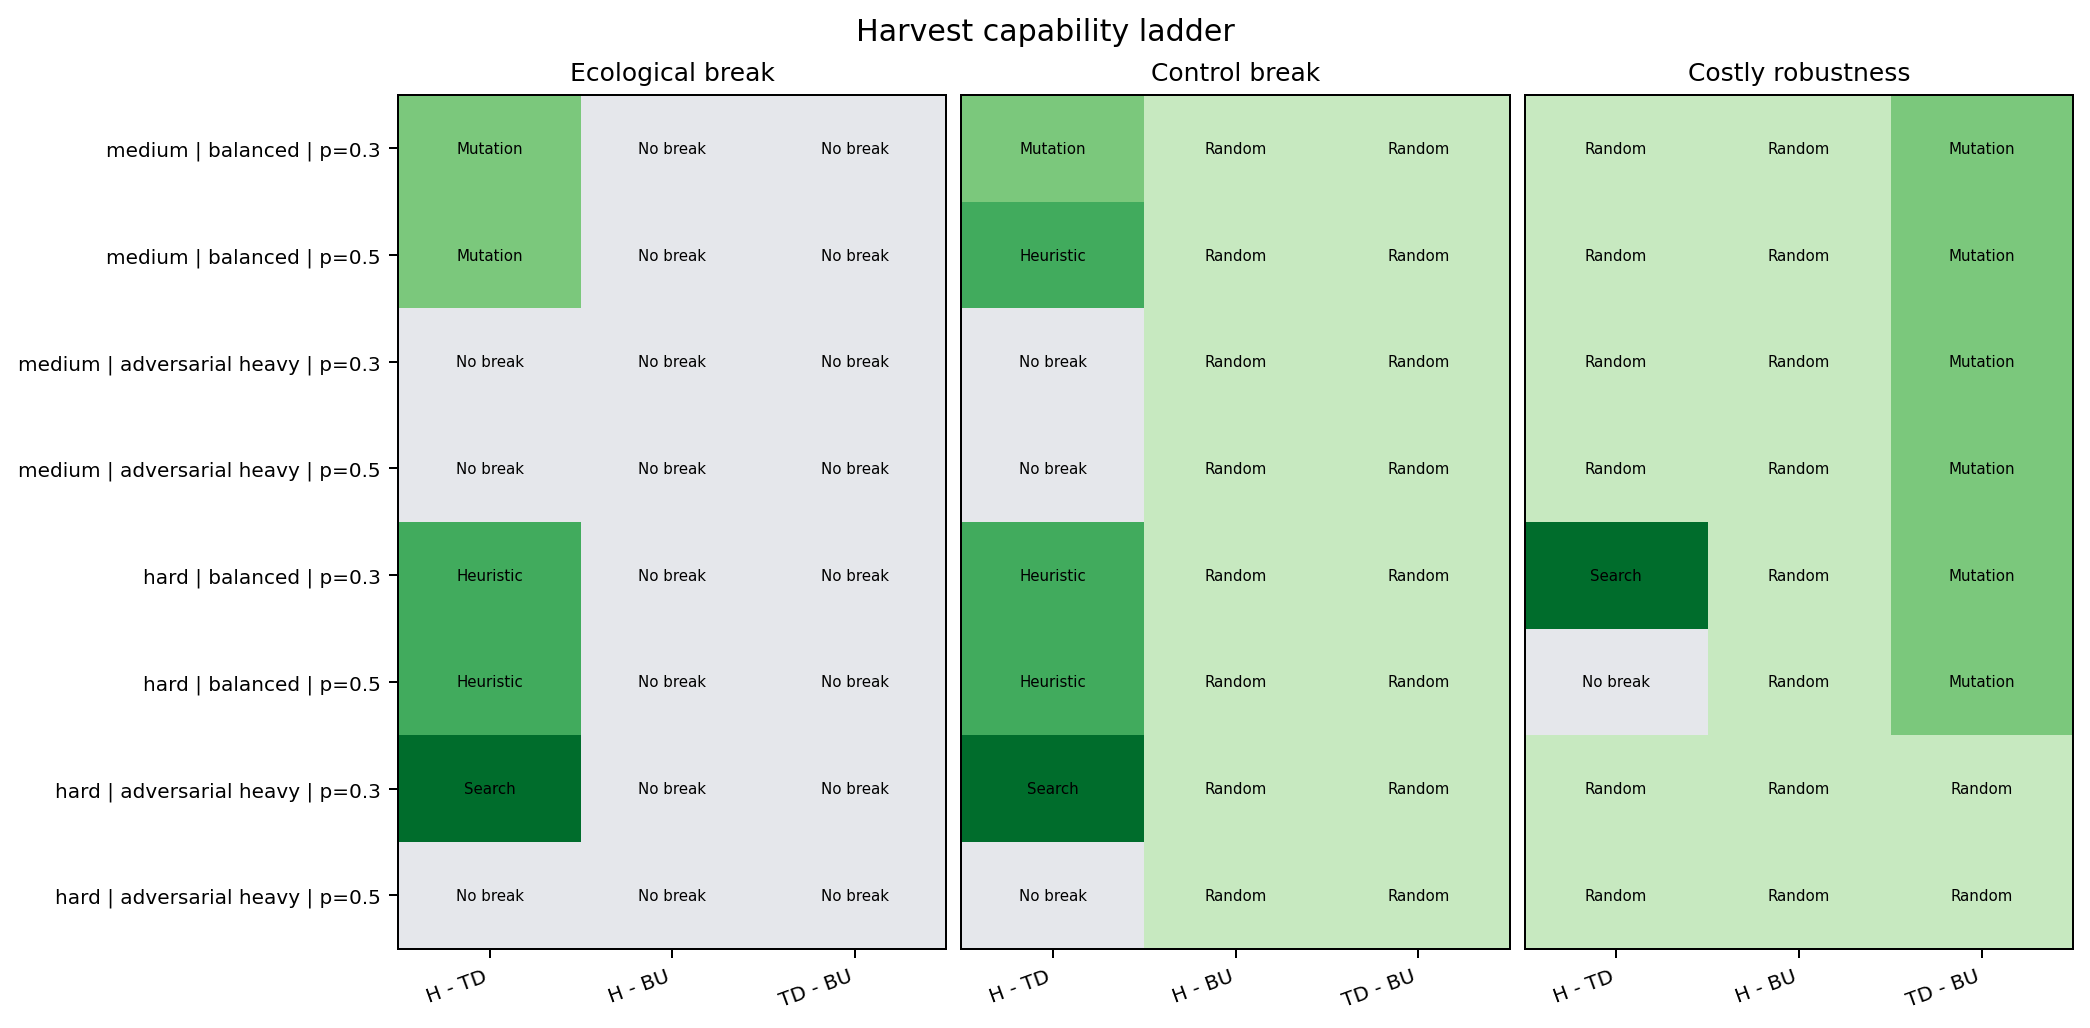
\includegraphics[width=\linewidth]{figures/harvest_capability_ladder_stageB_capability_ladder.png}
  \caption{Capability-ladder summary for Harvest Commons. Each cell reports the first attacker rung at which a pairwise architecture contrast loses its ecological advantage, loses its neighborhood-overharvest advantage, or crosses the welfare-cost threshold. Abbreviations are \texttt{H} for \texttt{hybrid}, \texttt{TD} for \texttt{top\_down\_only}, and \texttt{BU} for \texttt{bottom\_up\_only}. The governed-versus-local-only contrasts remain ecologically stable across the full ladder, while the hybrid-versus-top-down margin is the more contested part of the ordering.}
  \label{fig:harvest_capability_ladder}
\end{figure}

\subsection{Welfare incidence}

The incidence summaries help interpret the welfare trade-off. For the confirmatory \texttt{hybrid - top\_down\_only} comparison, the per-tercile welfare deltas are modest across the board: averaged over the high-, mid-, and low-aggression groups, the mean welfare effects are approximately \(-0.0134\), \(-0.0168\), and \(-0.0379\), respectively. The targeted-agent view tells a similar story. For agents who are actually targeted by caps, the mean welfare delta is only \(-0.0227\), while the corresponding mean local-patch-health delta is \(+0.0468\). In other words, the incremental cost of moving from central-only to hybrid governance is not large in the same way as the architecture-versus-local-only contrast.

This distinction is important for interpretation. The larger welfare penalty in this study is the cost of restoring ecological control when moving away from local-only governance, not the cost of adding local coordination on top of an already functioning central architecture. Hybrid governance therefore appears less as a globally punitive architecture than as a modestly more interventionist extension of top-down control that yields additional ecological stability.

\begin{figure}[t]
  \centering
  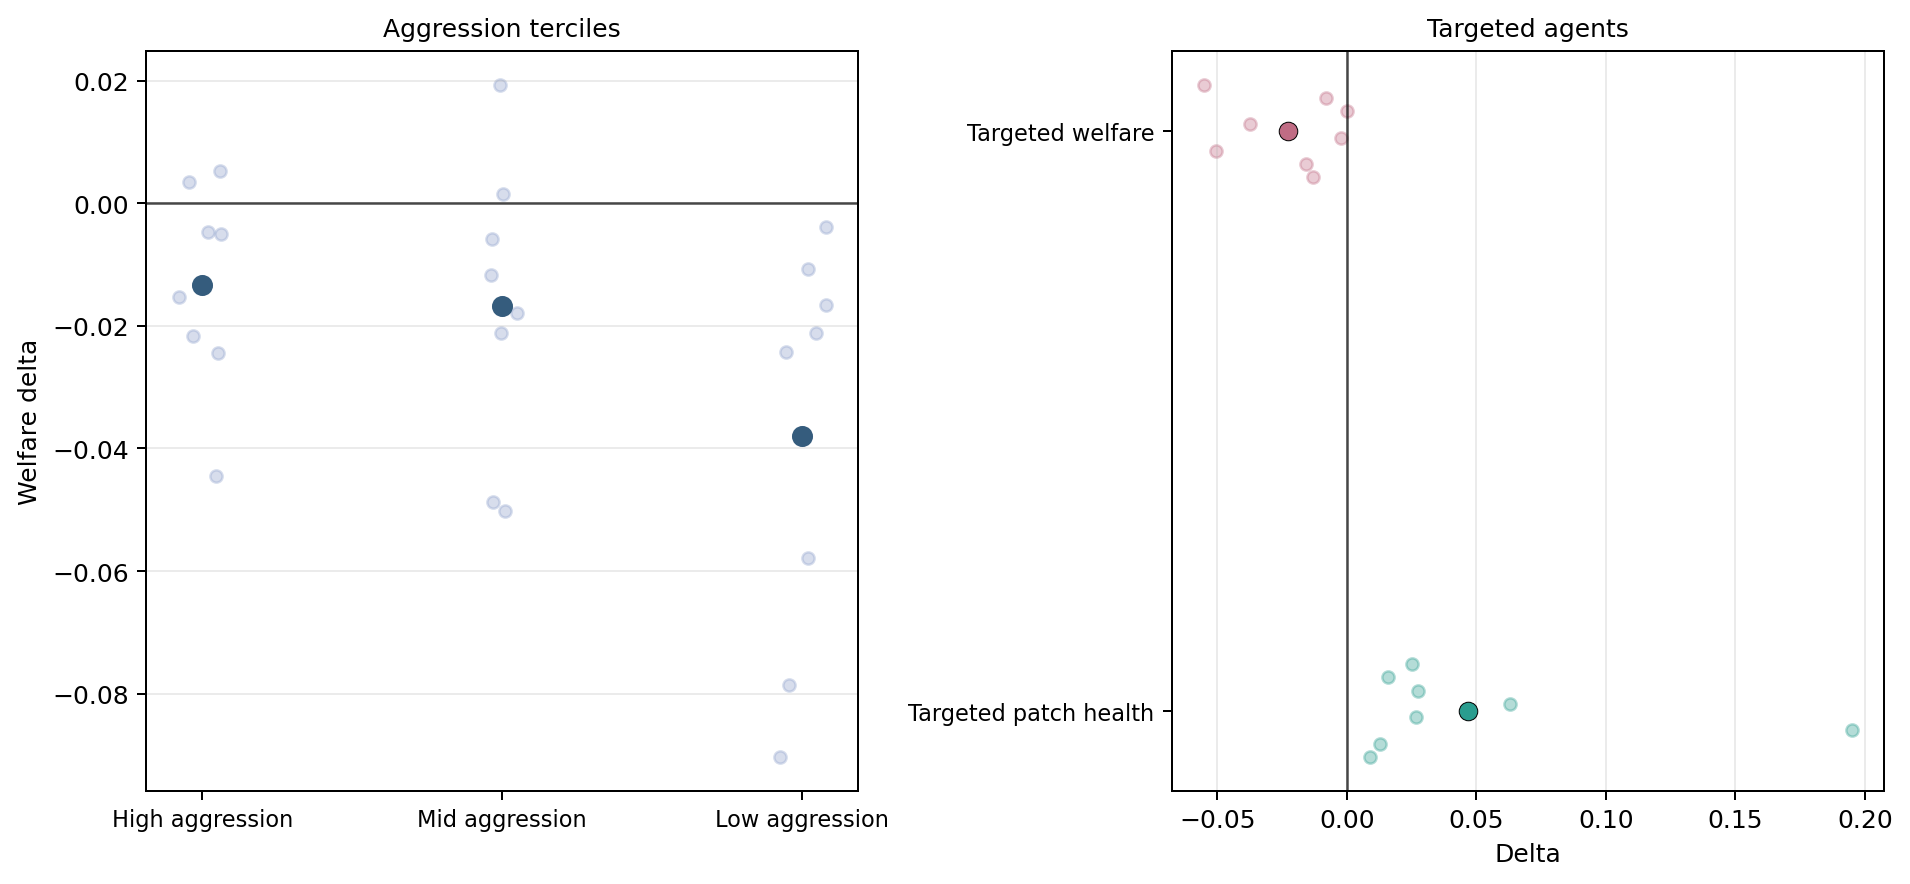
\includegraphics[width=\linewidth]{figures/harvest_architecture_stageC_welfare_incidence.png}
  \caption{Welfare-incidence summary for Harvest Commons. The left panel shows cell-level welfare deltas by aggression tercile for \texttt{hybrid - top\_down\_only}; the larger markers indicate tercile means. The right panel shows the same contrast for targeted agents, reporting both welfare and local patch-health deltas. Relative to top-down-only control, hybrid governance imposes a modest incremental welfare cost while improving local patch health.}
  \label{fig:harvest_incidence}
\end{figure}
